\chapter[Los n\'umeros de Bernoulli: un ejemplo del \'area de An\'alisis]{Los n\'umeros de Bernoulli: un ejemplo del \'area de An\'alisis Matem\'atico}
\label{CapituloBernoulli}

Cualquiera que haya estudiado un primer curso de C\'alculo conoce los desarrollos en serie de potencias de las funciones seno y coseno. No es tan conocido, y tampoco tan f\'acil, encontrar el desarrollo en serie de potencias de la funci\'on tangente. \'Este ser\'a nuestro objetivo. Sorprendentemente los coeficientes que aparecen tienen relaci\'on con muchos otros resultados en contextos que nada tienen que ver con la funci\'on tangente, tales como las f\'ormulas para sumar potencias de n\'umeros consecutivos. La mayor parte de este cap\'\i tulo se basa en \cite[Cap\'\i tulo 27]{Spivak}.

\section{Los n\'umeros de Bernoulli}

La funci\'on de variable compleja $$f(z)=\begin{cases} \displaystyle\frac{e^z-1}{z} & \text{si  } z\not=0\\
\hfill 1\hfill  & \text{si } z=0\end{cases}$$
es anal\'\i tica en todo el plano complejo (su desarrollo en serie de potencias es $1+z/2!+z^2/3!+\cdots$) y es no nula en el c\'\i rculo $|z|<2\pi$, por tanto la funci\'on $g(z)=1/f(z)$ tambi\'en es anal\'\i tica en este c\'\i rculo y puede desarrollarse como serie de potencias alrededor de $0$ (serie que tendr\'a radio de convergencia igual a $2\pi$). Podemos escribir entonces

\begin{equation}
\label{desarrollo}
\frac{z}{e^z-1}=\sum_{k=0}^\infty \frac{b_k}{k!}z^k.
\end{equation}

\begin{definicion} Los n\'umeros $b_k$ que aparecen en (\ref{desarrollo}) se llaman \emph{n\'umeros de Bernoulli}\footnote{\emph{Jacob Bernoulli}, Basilea, 1654-1705.}.
\end{definicion}

Como
$$z=\left(\sum_{k=0}^\infty\frac{b_k}{k!}z^k\right)\left(z+\frac{z^2}{2!}+\frac{z^3}{3!}+\cdots \right),$$
el coeficiente de $z^n$ en la derecha es $1$ para $n=1$ y cero para $n>1$,  es decir
$$b_0=1\quad \text{y}\quad  0=\sum_{k+i=n \atop k\geq 0,\,i\geq 1}\frac{b_k}{k!}\,\frac{1}{i!}=n!\sum_{k=0}^{n-1}{n\choose k}b_k,\  \text{ para } n>1,$$ de donde resulta la f\'ormula por recurrencia que, junto con el valor inicial $b_0=1$, permite  calcular los n\'umeros de Bernoulli:

\begin{equation}\label{RecurrenciaBernoulli}\sum_{k=0}^{n-1}{n\choose k}b_k=0,\ \ \text{para } n>1.\end{equation}

Notar que de aqu\'\i\ se sigue que los n\'umeros de Bernoulli $b_n$ son n\'umeros racionales, un hecho que no es inmediato de su definici\'on.

\section{La suma de las $n$ primeras potencias $p$-\'esimas}

Los n\'umeros de Bernoulli fueron introducidos originalmente por Jacob Bernoulli para dar una f\'ormula expl\'\i cita para la suma de las $n$ primeras potencias $p$-\'esimas de los n\'umeros naturales: $S_p(n)=1^p+2^p+\cdots +n^p$.

Comenzamos por un  resultado que tiene inter\'es en s\'\i\ mismo puesto que permite calcular $S_p(n)$ a partir de $S_j(n)$ para $j<p$.

\begin{proposicion}\label{RecurrenciaSumaPotencias} Sea $p\geq 0$. Entonces
$$S_p(n)=\frac{(n+1)^{p+1}-1}{p+1}-\frac{1}{p+1}\sum_{j=0}^{p-1}{p+1\choose j}S_j(n).$$
\end{proposicion}

\begin{demostracion}
Por la f\'ormula del binomio de Newton, para $i\geq 2$,
$$i^{p+1}=((i-1)+1)^{p+1}=\sum_{j=0}^{p+1}{p+1\choose j}(i-1)^j.$$
Sumando en $i$ desde $2$ hasta $n+1$ resulta que
\begin{eqnarray*}
S_{p+1}(n+1) &=& 1+\sum_{i=2}^{n+1}i^{p+1}=1+\sum_{i=2}^{n+1}\sum _{j=0}^{p+1}{p+1\choose j}(i-1)^j\\  &=& 1+\sum_{j=0}^{p+1}\sum_{i=2}^{n+1}{p+1\choose j}(i-1)^ j= 1+\sum_{j=0}^{p+1}{p+1\choose j}S_j(n)\\ &=& 1+S_{p+1}(n)+(p+1)S_p(n)+\sum_{j=0}^{p-1}{p+1\choose j}S_j(n).\end{eqnarray*}
Basta ahora despejar $S_p(n)$ y tener en cuenta que $S_{p+1}(n+1)-S_{p+1}(n)=(n+1)^{p+1}$.
\end{demostracion}

Utilizando esta f\'ormula por recurrencia y el valor inicial $S_0(n)=n$ podemos calcular las primeras f\'ormulas de $S_p(n)$. En la Tabla \ref{potencias} damos estas f\'ormulas para $p\leq 5$.


\begin{table}\begin{center}
\begin{tabular}{|c|l|}
\hline
\multicolumn{2}{|c|}{\rule[-3mm]{0mm}{8mm} $S_p(n)=1^p+2^p+\cdots +n^p$}\\
\hline
$p$ & \multicolumn{1}{c|}{\rule[-2mm]{0mm}{6mm} $S_p(n)$} \\
\hline
\hline
\rule[-2mm]{0mm}{6mm} 1& $\frac{1}{2}n(n+1)$\\
\hline
\rule[-2mm]{0mm}{6mm} 2& $\frac{1}{6}n(n+1)(2n+1)$\\
\hline
\rule[-2mm]{0mm}{6mm} 3& $\frac{1}{4}n^2(n+1)^2$\\
\hline
\rule[-2mm]{0mm}{6mm} 4& $\frac{1}{30}n(n+1)(2n+1)(3n^2+3n-1)$\\
\hline
\rule[-2mm]{0mm}{6mm} 5& $\frac{1}{12}n^2(n+1)^2(2n^2+2n-1)$\\
\hline
\end{tabular}\end{center}
\caption{\label{potencias} Las primeras f\'ormulas para $S_p(n)$.}
\end{table}

De la proposici\'on anterior se sigue tambi\'en mediante un sencillo argumento inductivo que $S_p(n)$ viene dado por un polinomio en $n$ de grado $p+1$ y, m\'as a\'un, que  su t\'ermino principal es $\frac{n^{p+1}}{p+1}$. En realidad este hecho es f\'acilmente explicable: la funci\'on $f(x)=x^p$ es convexa para $p\geq 1$. La suma $S_p(n)$ no es m\'as que el \'area sombreada en la Figura \ref{funciones}, situada entre las gr\'aficas de las funciones $f(x)=(x+1)^p$ y $g(x)=x^p$. Es claro entonces que $$\int_0^nx^p\,\mathrm{d}x<S_p(n)<\int_0^n(x+1)^p\,\mathrm{d}x ,$$
es decir $$\frac{n^{p+1}}{p+1}<S_p(n)<\frac{(n+1)^{p+1}}{p+1}=\frac{n^{p+1}}{p+1}+\cdots.$$

\begin{figure}
\begin{center}
\scalebox{0.8}{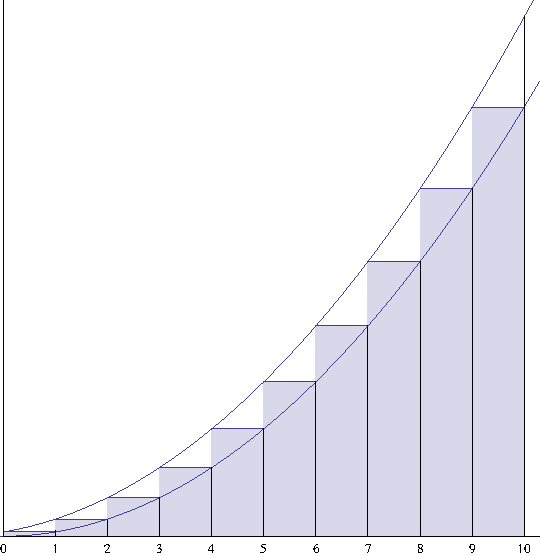
\includegraphics{Riemann.pdf}}
\end{center}
\caption{\label{funciones} Las funciones $f(x)=(x+1)^p$ y $g(x)=x^p$.}
\end{figure}

A continuaci\'on damos la f\'ormula expl\'\i cita para $S_p(n)$. En el Ap\'endice \ref{Ars Conjectandi} reproducimos una p\'agina del libro de J. Bernoulli \emph{Ars Conjectandi}, publicado en 1713, en la que se pueden ver las f\'ormulas de $S_p(n)$ para $p\leq 10$. Bernoulli contin\'ua diciendo que, en vista de estas f\'ormulas, cualquiera puede continuar la tabla. Necesitaremos el siguiente resultado t\'ecnico.

\begin{lema} Si $0\leq k\leq j\leq p$,
$$\frac{1}{j+1}{p+1\choose j}{j+1\choose k}=\frac{1}{j-k+1}{p+1\choose p-j+k+1}{p-j+k+1\choose k}.$$\end{lema}

\begin{demostracion}
La parte de la izquierda es igual a
\begin{eqnarray*}&\frac{1}{j+1}\,\frac{(p+1)!}{j!\,(p-j+1)!}\,\frac{(j+1)!}{k!\,(j-k+1)!}
=\frac{1}{j-k+1}\,\frac{(p+1)!}{(j-k)!\,(p-j+k+1)!}\,\frac{(p-j+k+1)!}{k!\,(p-j+1)!},&
\end{eqnarray*}
que es justamente la parte de la derecha.
\end{demostracion}

\begin{teorema} Sea $p\geq 1$. Entonces
\begin{equation}\label{FormulaSumaPotencias} S_p(n)=\frac{1}{p+1}\sum_{k=0}^p{p+1\choose k}b_k(n+1)^{p-k+1}.\end{equation}
\end{teorema}

\begin{demostracion}
Razonamos por inducci\'on sobre $p$, comprob\'andose de forma inmediata el caso $p=1$. Si $p\geq 2$, aplicando la Proposici\'on \ref{RecurrenciaSumaPotencias}, la hip\'otesis inductiva y el lema anterior, resulta que
\begin{eqnarray*}
&&\textstyle S_p(n)=\frac{(n+1)^{p+1}}{p+1}-\frac{n+1}{p+1}-\frac{1}{p+1}\sum_{j=1}^{p-1}{p+1\choose j}S_j(n)\\
&=&\textstyle \frac{(n+1)^{p+1}}{p+1}-\frac{n+1}{p+1}-\frac{1}{p+1}\sum_{1\leq j\leq p-1\atop 0\leq k\leq j}\frac{1}{j+1}{p+1\choose j}{j+1\choose k}b_k(n+1)^{j-k+1}\\
&=&\textstyle \frac{(n+1)^{p+1}}{p+1}-\frac{1}{p+1}\sum_{0\leq j\leq p-1\atop 0\leq k\leq j}\frac{1}{j+1}{p+1\choose j}{j+1\choose k}b_k(n+1)^{j-k+1}\\
&=&\textstyle \frac{(n+1)^{p+1}}{p+1}-\frac{1}{p+1}\sum_{0\leq j\leq p-1\atop 0\leq k\leq j}\frac{1}{j-k+1}{p+1\choose p-j+k+1}{p-j+k+1\choose k}b_k(n+1)^{j-k+1}.
\end{eqnarray*}
A continuaci\'on hacemos el cambio de \'\i ndice de sumaci\'on $h=p-j+k$. Como $j$ var\'\i a entre $k$ y $p-1$, $h$ var\'\i a entre $k+1$ y $p$ o, si se prefiere, $h$ var\'\i a de $1$ a $p$ y $k$ de $0$ a $h-1$. As\'\i\ tenemos que
\begin{eqnarray*}
&&\textstyle S_p(n)=\frac{(n+1)^{p+1}}{p+1}-\frac{1}{p+1}\sum_{1\leq h\leq p\atop 0\leq k\leq h-1}\frac{1}{p-h+1}{p+1\choose h+1}{h+1\choose k}b_k(n+1)^{p-h+1}\\
&=&\textstyle  \frac{(n+1)^{p+1}}{p+1}-\frac{1}{p+1}\sum_{h=1}^p\frac{1}{p-h+1}{p+1\choose h+1}\left(\sum_{k=0}^{h-1}{h+1\choose k}b_k\right) (n+1)^{p-h+1}.
\end{eqnarray*}
De (\ref{RecurrenciaBernoulli}) deducimos que $\sum_{k=0}^{h-1}{h+1\choose k}b_k=-{h+1\choose h}b_h=-(h+1)b_h$. Como adem\'as $\frac{h+1}{p-h+1}{p+1\choose h+1}={p+1\choose h}$ concluimos que
\begin{eqnarray*}S_p(n)&=& \frac{(n+1)^{p+1}}{p+1}+\frac{1}{p+1}\sum_{h=1}^p{p+1\choose h}b_h(n+1)^{p-h+1}\\&=&
\frac{1}{p+1}\sum_{h=0}^p{p+1\choose h}b_h(n+1)^{p-h+1},\end{eqnarray*}
que es lo que quer\'\i amos demostrar.
\end{demostracion}

\begin{observacion*} Si se prefiere, la f\'ormula (\ref{FormulaSumaPotencias}) tambi\'en se puede expresar como un polinomio en $n$ sin m\'as que notar que
\begin{eqnarray*}S_p(n)&=&n^p+S_p(n-1)=n^p+\frac{1}{p+1}\sum_{k=0}^p{p+1\choose k}b_kn^{p-k+1}\\ &=&
\frac{n^{p+1}}{p+1}+\frac{n^p}{2}+\frac{1}{p+1}\sum_{k=2}^p{p+1\choose k}b_kn^{p-k+1}.\end{eqnarray*}
\end{observacion*}

\section{El desarrollo en serie de potencias de la funci\'on tangente}

Es inmediato comprobar que
$$
g(z)=\frac{z}{e^z-1}=-\frac{z}{2}+\frac{z}{2}\,\frac{e^z+1}{e^z-1} \quad\text{y}\quad
\frac{e^{-z}+1}{e^{-z}-1}=-\frac{e^z+1}{e^z-1},$$
lo que significa que $g(z)=-z/2+h(z)$, donde $\displaystyle h(z)=\frac{z}{2}\,\frac{e^z+1}{e^z-1}$ es una funci\'on par. Las potencias impares en el desarrollo en serie de potencias de $h(z)$ tienen por  tanto coeficientes nulos, es decir, $b_1=-1/2$ y $b_n=0$ para todo n\'umero impar $n>1$.

Resulta entonces que

\begin{equation}\label{funcionpar}\sum_{n=0}^\infty\frac{b_{2n}}{(2n)!}z^{2n}=g(z)+\frac{z}{2}=
\frac{z}{2}\,\frac{e^z+1}{e^z-1}=\frac{z}{2}\,\frac{e^{z/2}+e^{-z/2}}{e^{z/2}-e^{-z/2}}.
\end{equation}

Recordemos que
$$\ctg z=i\,\frac{e^{iz}+e^{-iz}}{e^{iz}-e^{-iz}},$$
entonces, sustituyendo $z$ por $2iz$ en (\ref{funcionpar}) queda:

$$\sum_{n=0}^\infty (-1)^n\frac{b_{2n}}{(2n)!}2^{2n}z^{2n}=iz\frac{e^{iz}+e^{-iz}}{e^{iz}-e^{-iz}}=z\ctg z,$$
de donde resulta el desarrollo en serie de Laurent de la funci\'on cotangente alrededor de $0$:

\begin{equation}\label{ctg}\ctg z=\frac{1}{z}+\sum_{n=1}^\infty (-1)^n\frac{b_{2n}}{(2n)!}2^{2n}z^{2n-1}.
\end{equation}

Finalmente, se tiene que $\tg z=\ctg z-2\ctg 2z$ (ver el Ejercicio \ref{ej.tangente} en el Ap\'endice A)  as\'\i\ que, sin m\'as que usar (\ref{ctg}), se obtiene el desarrollo en serie de potencias de la funci\'on tangente.

\begin{teorema}\label{desarrollo tangente} La funci\'on tangente tiene el siguiente desarrollo en serie de potencias alrededor del cero:
$$\tg z=\sum_{n=1}^\infty (-1)^{n-1}\frac{b_{2n}}{(2n)!}2^{2n}(2^{2n}-1)z^{2n-1}.$$
\end{teorema}

Como corolario inmediato podemos calcular el valor de las derivadas sucesivas de la funci\'on tangente en el cero, un resultado muy dif\'\i cil de obtener (si no imposible) por derivaci\'on directa.

\begin{corolario} Sea $f(x)=\tg x$. Entonces, si $k\geq 1$,
$$f^{(k)}(0)=(-1)^{(k+1)/2}\frac{b_{k+1}}{k+1}2^{k+1}(2^{k+1}-1).$$
\end{corolario}

\begin{demostracion} Basta tener en cuenta que el desarrollo del Teorema \ref{desarrollo tangente} no es m\'as que la serie de McLaurin de la funci\'on tangente y, por tanto,
$$f(x)=\sum_{k=0}^\infty\frac{f^{(k)}(0)}{k!}x^k=
\sum_{k=1}^\infty (-1)^{(k+1)/2}\frac{b_{k+1}}{(k+1)!}2^{k+1}(2^{k+1}-1)x^k.$$
El resultado se sigue igualando los coeficientes de $x^k$.
\end{demostracion}

\section{N\'umeros de Fibonacci y n\'umeros de Bernoulli}

Los n\'umeros de Fibonacci y de Bernoulli estudiados en este trabajo, as\'\i\ como muchas de sus generalizaciones y polinomios asociados, est\'an relacionados mediante numerosas f\'ormulas. S\'olo daremos una de ellas, pueden encontrarse muchas otras en \cite{Byrd} y en sus referencias.

\begin{teorema} Para todo $n\geq 0$ se cumple que
$$\Phi^n=\sum_{k=0}^n {n\choose k}(-\sqrt 5)^k\frac{F_{n-k+1}}{n-k+1}b_k.$$
\end{teorema}

\begin{demostracion}
La f\'ormula a demostrar puede reescribirse como
$$\sum_{i+k=n+1\atop k\geq 0,\, i\geq 1}\frac{F_i}{i!}\frac{(-\sqrt 5)^kb_k}{k!}=\frac{\Phi^n}{n!}.$$
La suma de la izquierda no es m\'as que el coeficiente de $z^{n+1}$ en el desarrollo en serie de potencias del producto
$$\left(\sum_{i\geq 1}\frac{F_i}{i!}z^i\right)\left(\sum_{k\geq 0}\frac{(-\sqrt 5)^kb_k}{k!} z^k\right).$$
La segunda serie de potencias en este producto es la de la funci\'on $\displaystyle\frac{-\sqrt 5 z}{e^{-\sqrt 5 z}-1}$ mientras que  la primera define la funci\'on $\rule[-16pt]{0pt}{26pt}\displaystyle \smash{F(z)=\frac{e^{\Phi z}-e^{(-1/\Phi)z}}{\sqrt 5}}$ (esto se puede comprobar directamente a partir de la f\'ormula expl\'\i cita para los n\'umeros de Fibonacci o, mejor aun, viendo por derivaci\'on directa de la serie que $F''-F'-F=0$ y resolviendo esta ecuaci\'on diferencial con los valores iniciales $F(0)=0$, $F'(0)=1$).

Finalmente observamos que
$$ \frac{e^{\Phi z}-e^{(-1/\Phi)z}}{\sqrt 5} \frac{-\sqrt 5 z}{e^{-\sqrt 5 z}-1} = 
\frac{z(e^{\Phi z}-e^{(-1/\Phi)z})}{1-e^{-(\Phi+\frac{1}{\Phi})z}}=ze^{\Phi z},$$
que al desarrollar en serie de potencias tiene como coeficiente de $z^{n+1}$ el t\'ermino deseado $\frac{\Phi^n}{n!}$.
\end{demostracion} 